%-------------------------------------------------------------------------------
\section{Design}
%-------------------------------------------------------------------------------

\subsection{Specifying Decorrelation Policies}
\lyt{FIGURE HERE} 

\begin{figure}
\begin{lstlisting}[language=Rust]
 pub enum GeneratePolicy {
     Random,
     Default,
     Custom(FnMut(ColumnValue) -> ColumnValue),
     ForeignKey, 
 }
 pub enum GhostColumnPolicy {
     CloneAll,
     CloneOne(gp: GeneratePolicy),
     Generate(gp: GeneratePolicy),
 }
 pub type GhostPolicy = 
    HashMap<Column, GhostColumnPolicy>;
 pub type EntityGhostPolicies = 
    HashMap<EntityName, GhostPolicy>;

pub enum DecorrelationPolicy {
     NoDecorRemove,
     NoDecorRetain,
     NoDecorSensitivity(f64),
     Decor,
 }
 pub struct KeyRelationship {
     child: EntityName,
     parent: EntityName,
     column_name: String,
     decorrelation_policy: DecorrelationPolicy,
 }
 pub type ApplicationPolicy = 
    (EntityGhostPolicies, Vec<KeyRelationship>);
\end{lstlisting}
    \caption{\sys{}-provided types to specify key relationships and ghost generation policies.
    \lyt{An actual instance of this policy is here: \url{https://github.com/tslilyai/gdpr/blob/master/decor/applications/lobsters/microbenchmarks/policy.rs}}}
\end{figure}

Application data is structured as tables, each representing a different \emph{table entity} type,
e.g.,\ stories, users, or votes. Table columns act as foreign keys to other table entities, or as
abstract keys that refer to abstract non-table entities (e.g.,\ a \texttt{thread\_id} comments column). 
Key relationships represent correlations between entity types.

\sys{} represents instances of key-based relationships between entities as the edges of a graph,
where the nodes are the entity instances: child entities are connected to parents via an instance of
a foreign or abstract key relationship. In the following, an \emph{edge} refers to an instance of a
foreign or abstract key relationship.

The developer provides a two-part specification to \sys{}: 
\begin{enumerate}
    \item Ghost entity generation policies on entity types, and
    \item Decorrelation policies for foreign/abstract key relationships specifying if and how
        instances of these edge types should be decorrelated.
\end{enumerate}

\noindent The following describes the options for the different parts of the developer-provided
specification in more detail.

\subsubsection{Ghost Entity Generation}
Developers can choose between the following ghost generation policies, which apply at 
per-column granularity.
\begin{itemize}
    \item \textbf{Cloned:} All ghosts have the same value as the original entity for this column.
        Recorrelation returns an entity with the original value.

    \item \textbf{Generated:} All ghosts have a generated value for this column. Generated values are
chosen to be random, a default value, or generated from the original value via a function provided by the developer.
        If the developer provides a reversible function (e.g.,\ has encrypted the original value
        with a user-specific key), then the original value is restored upon
        recorrelation; otherwise, recorrelation returns a generated value in place of the original.

        If the column represents a foreign key into another table, then either the referenced table must 
        have a ghost generation policy, or the foreign key is set to an existing entity or placeholder ghost (e.g.,
        the foreign key is set to point to ``deleted story''). It is up to the developer to ensure
        referential integrity in the latter case.

\item \textbf{Single Clone, Generated Remainder:} One ghost has the same value as the original
        entity; all other ghosts have generated values. Recorrelation returns an entity with the original value.
\end{itemize}


\subsubsection{Decorrelation Policies}

\paragraph{Policy 1: Decorrelate.}
Application developers specify that the relationship may be decorrelated.
\sys{} generates a ghost parent entity for the child entity according to the parent entity's ghost
generation policy, replacing the child's key with the new ghost parent key.

Resubscription (and recorrelation) removes any created ghost entities and restores the relationship
back to the original parent key instance.

%\lyt{There could also be an option to "decorrelate the minimum amount possible to reach a
%certain sensitivity threshold"; not sure if it's useful since the edges can already be
%decorrelated.}
%
\paragraph{Policy 2: Do not decorrelate.}
Application developers specify that this foreign or abstract key relationship cannot be decorrelated.
Developers select from the following subpolicy options: 
\begin{itemize}
    \item \textbf{Delete}: The child entity and its dependencies are deleted. This option should be
        selected if this type of key relationship cannot be decorrelated while retaining application
        semantics, but keeping the relationship would reveal too much identifying information.
        Upon recorrelation, however, these entities cannot be restored.

    \item \textbf{Retain}: Nothing is done on either side of the
        relationship. This option should only be selected if the developer knows that the
        relationship cannot leak identifying information.

    \item \textbf{Achieve sensitivity threshold $0 \le \sigma \le 1$}:
        A sensitivity threshold for an foreign/abstract key relationships specifies the maximum
        proportion of edge instances of a relationship type that may connect to \emph{sensitive}
        entities (i.e.,\ entities transitively correlated to the initial entity being decorrelated). 

        At a high level, the sensitivity threshold for a particular edge type estimates how much identifying
        information may leak from edge instances of that type.  For any given edge type, developers can
        determine an appropriate sensitivity threshold by approximating how much identifying information
        may be leaked if edges of this type with the same parent key \emph{all} correlate (even indirectly)
        back to the entity being decorrelated. In other words, what happens if all children of edges of this
        type (with the same parent) are sensitive?

        For example, consider the foreign key relationship from stories to tags. If all
        the stories tagged with the same parent tag in the entity graph were written by some
        (unsubscribed) user, would the story-tag correlation be problematic? The answer may be yes: 
        perhaps tags are customizable by the user, and any story with that tag will clearly
        belong to the unsubscribed user. In other cases, the answer may be no: even though the tag is only
        correlated with sensitive stories, the tag indicates nothing about who may have authored the stories.

        For many cases, the answer may lie somewhere in the middle: it is problematic if \emph{all} of
        children of edge of this type are sensitive, but perhaps it is acceptable if only a fraction of
        children of this edge type are sensitive. The maximum value for this fraction is the sensitivity threshold.
        For example, a reasonable sensitivity threshold might be $\sigma = 0.1$ for stories-tag key relationships:
        less than 10\% of all stories with a specific tag key should have been correlated (even
        indirectly) with an (unsubscribed) user. 

        \sys{} either generates ghost children entities with this edge type until the
        sensitivity threshold is met (if a ghost generation policy is specified for the child type); upon
        resubscription, \sys{} removes any generated ghost entities and edges.
        Note that if the generated ghosts are easily distinguished from actual entities, there is
        little privacy benefit from generating ghost entities to meet the threshold.

        If the children entity type has no associated ghost generation policy, \sys{} removes
        sensitive children and their dependencies until the threshold is met.  Upon recorrelation,
        however, these entities cannot be restored.

        If $\sigma = 0$, then this corresponds to removing all edges of this type
        with sensitive children (equivalent to a Delete policy); if $\sigma = 1$, \sys{} does
        nothing (equivalent to a Retain policy).
    \end{itemize}

\subsubsection{\sys{}'s Execution Algorithm}
Given this specification and an entity to be decorrelated as input, \sys{} acts as follows:
\begin{enumerate}
    \item \textbf{Parent-Child Traversal:} \sys{} traverses the entity graph starting from the input entity,
        going down parent to child edges (and halting if it detects a cycle).  As it traverses,
        \sys{} collects the edges it has traversed. 
    
    \item \textbf{Parent-Child Decorrelation:} Post-traversal, \sys{} acts on each edge instance
        according to the specified decorrelation relationship policy for that edge's type: if no
        policy is specified, \sys{} does nothing. If edges can be decorrelated, \sys{} generates
        ghost parent entities and new edges between child and ghost parent entities using the
        appropriate ghost entity generation policy. If edges cannot be decorrelated and should be
        retained or deleted, \sys{} does nothing or removes the child and edge respectively. 
    
        If there is a sensitivity threshold for the edge's type, \sys{} ensures the
        sensitivity of the edge is below $t$'s threshold, providing the edge type and the edge's
        parent key to the procedure described in Section~\ref{sensitivity_algo}. 

    \item \textbf{Child-Parent Decorrelation:} Next, \sys{} takes the children of all traversed edge
        instances, and considers the set of edges from these children to other parents
        \emph{not} traversed by \sys{} during the decorrelation phase. (In other words, these
        children entities have multiple key relationships to several parent entities, one of
        which is connected via a chain of parent-child edges to the input entity).

        Intuitively, children of edges traversed by \sys{} share a connection with the initial
        entity being decorrelated. Edges \emph{from} these children to other parent entities may
        thus leak sensitive identifying information. 

        \sys{} acts on these edges according to the specified decorrelation relationship policy for
        each edge's type. If these edges can be decorrelated, \sys{} generates ghost parent entities
        for each sensitive child.  If these edges cannot be decorrelated and should be retained or
        deleted, \sys{} does nothing or removes the child and edge respectively. 
        
        \lyt{Note: edge policies should take account the \emph{direction} of the edge
        (whether we're considering sensitive child->parent, or sensitive parent->child). We need
        this to allow policies that decorrelate a message from one unsubscribing user while still retaining the correlation
        to another subscribed user.}

        Otherwise, if there is a sensitivity threshold for the edge type, then \sys{} limits the
        proportion of edges of that type that connect to sensitive entities (the children of
        traversed edge instances) to below the threshold. 
        For each edge with type $t$ in this set of edges, \sys{} ensures the
        sensitivity of the edge is below $t$'s sensitivity threshold, providing the edge type and the edge's
        parent key to the procedure described in Section~\ref{sensitivity_algo}. 
\end{enumerate}

\subsubsection{Achieving the Sensitivity Threshold}
\label{sensitivity_algo}
Let $E$ be the subset of edges traversed by \sys{} in Step 1 of execution. 
Given an edge type $t$ with sensitivity threshold $\sigma_t$, and a parent key $k$ of an instance of
edge type $t$, 
    \begin{itemize}
        \item \sys{} computes $N_{sensitive}$, the number of edges of type $t$ with parent $k$ in the entity graph that share 
            a child node with edges in $E$.
        \item \sys{} computes $N_{all}$, the total number of edges of type $t$ with parent $k$
            in the entity graph of edge.
        \item \sys{} computes $N_{sensitive}/N_{all}$, the \emph{sensitivity} of edges of type $t$
            with parent $k$.
        \item If the sensitivity exceeds $\sigma_t$ and the child entity type has an associated ghost entity policy, \sys{}
            generates ghost children and edges of type $t$ from these children to parent
            key $k$. This lowers the sensitivity by increasing $N_{all}$.
        \item Otherwise, if the sensitivity exceeds $\sigma_t$ but ghosts cannot be generated,
            \sys{} removes the children of edges in $E_t$ with parent $k$, thus lowering the
            sensitivity by lowering $N_{sensitive}$.
    \end{itemize}

Note that the initial sensitivity for an edge of type $t$ with parent $k$ from Step 2 (parent-child
decorrelation) is 1! Because \sys{} traverses from parent to child, if one edge of type $t$ with
parent $k$ was collected by \sys{}, then \emph{all} edges of type $t$ with parent $k$ were collected
by \sys{}. 

However, the initial sensitivity for an edge of type $t$ with parent $k$ from Step 3 (child-parent
decorrelation) may be very low: other parents of children touched by \sys{} may have many
non-sensitive children (e.g.,\ a tag may have many stories not authored by the user being
decorrelated).

\begin{figure}[t!]
    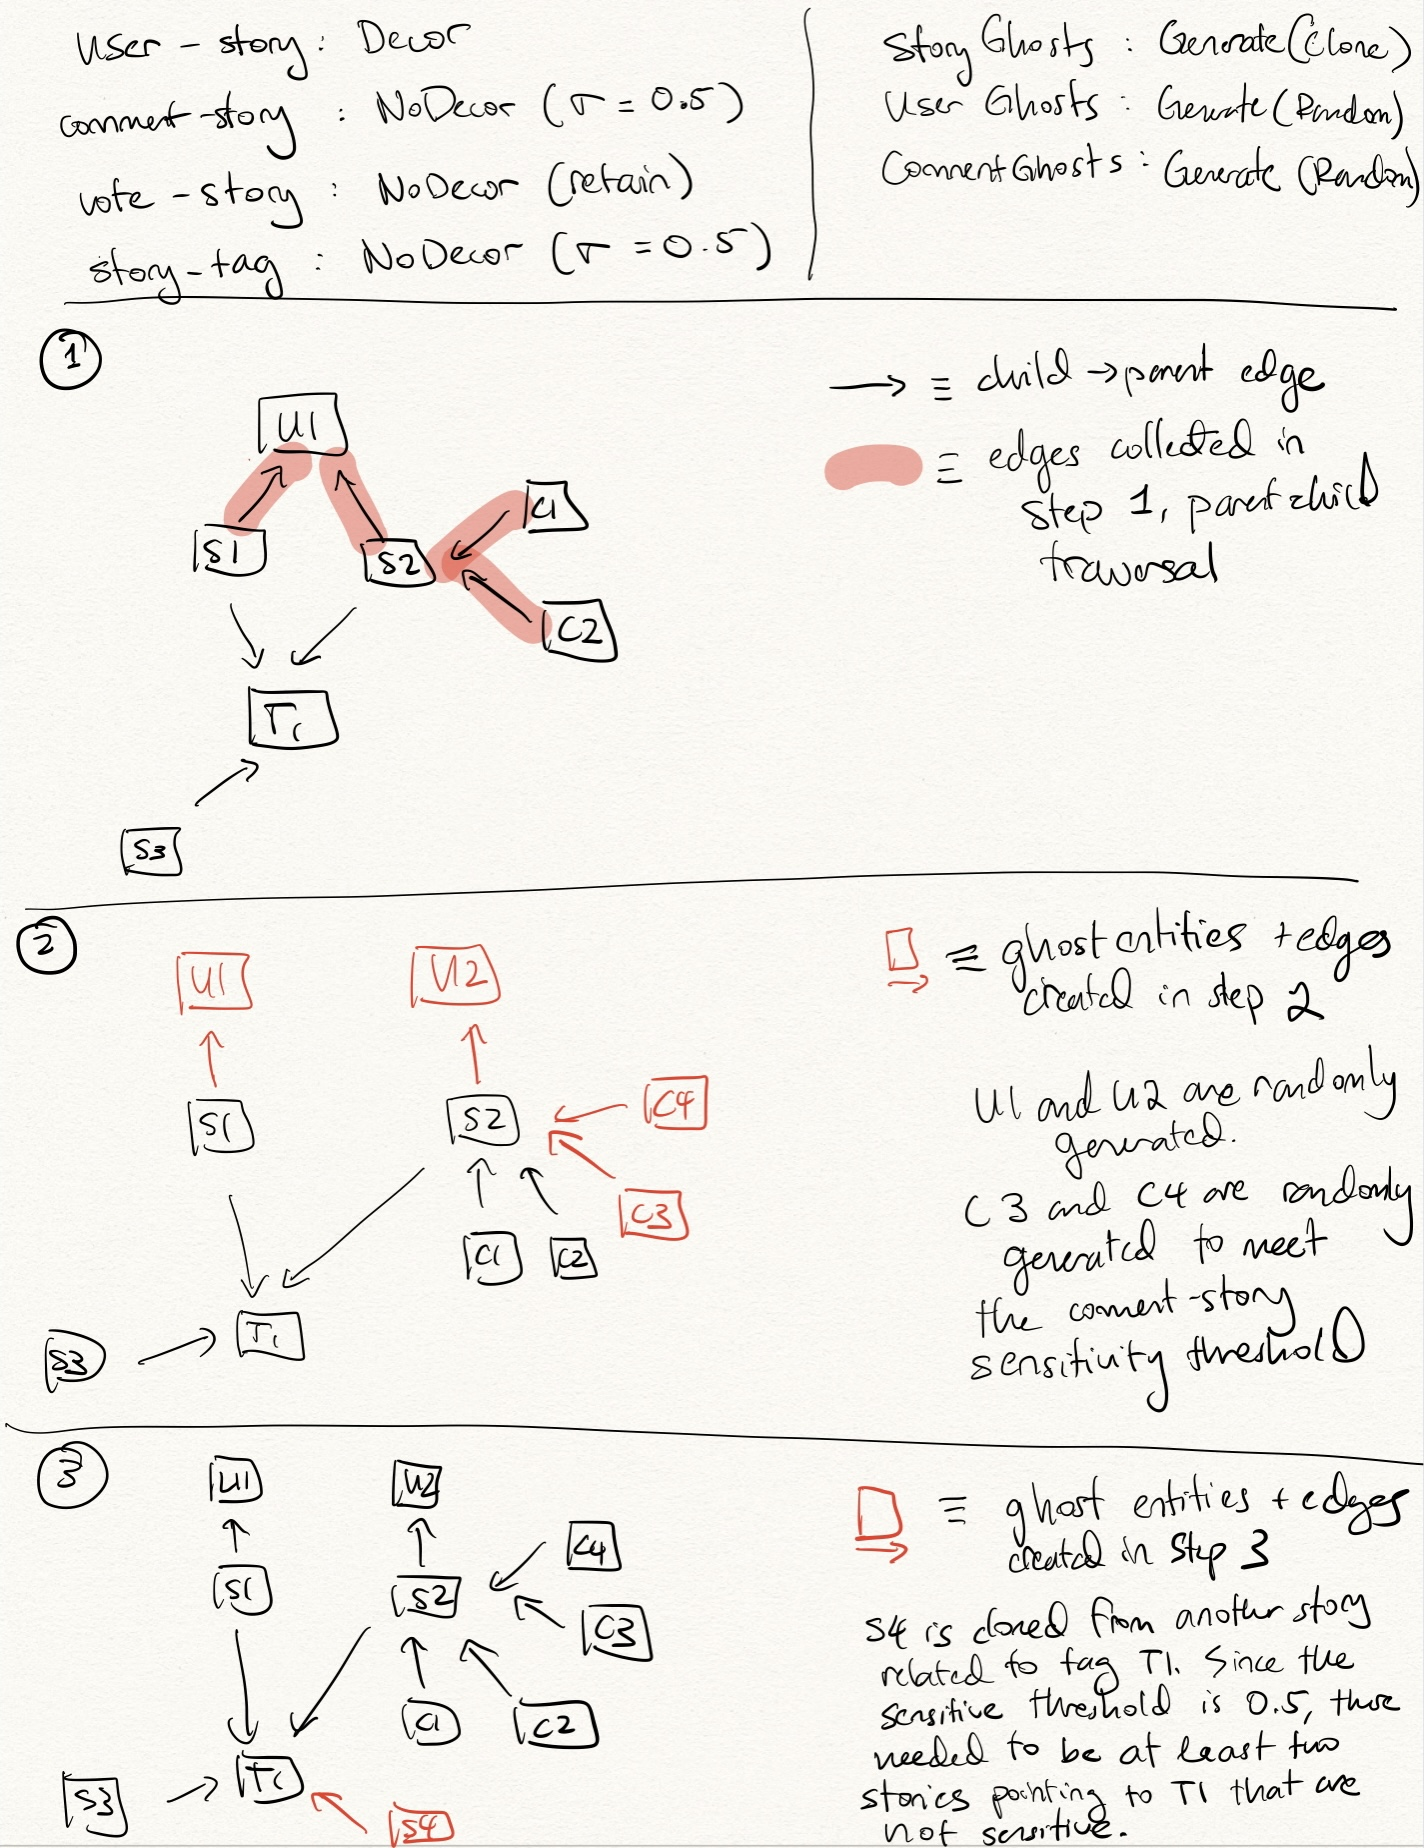
\includegraphics[width=.5\textwidth]{img/algo}
    \caption{Examples of \sys{}'s execution.}
    %different decorrelation policies. (a) full
    %decorrelation; (b) only direct user decorrelation; (c) decorrelation of stories clustered around tags with threshold 0.25}
\end{figure}

%\paragraph{Example policy.}
%We can imagine an application tin which only the sum of votes per story is ever queried by the application; clusters of
%votes around stories can therefore remain without leaking identifying information, and are thus
%assigned Policy 1, ``Do Not Decorrelate (Retain)''. 
%Decorrelation does propagate to the votes themselves, which are clustered by a \texttt{location} attribute; 
%this cluster by location can have a different decorrelation policy that generates ghost locations by
%randomizing the location, breaking up the cluster. 
%


\subsection{Maintaining aggregate accuracy.}
\sys{} optionally allows for entities to be decorrelated without affecting queries which
specifically return aggregation results.

Queries that specifically perform aggregations and return statistical measures (e.g.,
the count of number of users in the system, or the number of stories per user), can return
significantly different results. This affects the utility of the data for the application: for
example, if the application relies on the number of stories per tag to determine hot topics, these
would be heavily changed if ghost tags were created.  In addition, the adversary may learn which
entities are ghosts: for example, an abnormally low count of stories per tag might indicate to an
adversary that these tags are ghost tags.  \lyt{But perhaps it's ok if an adversary can tell what's
a ghost, as long as it can't tell which user each ghost is correlated with.}

\sys{} stores and separately updates answers to aggregation queries;
these answers are updated when queries update the data tables, and these queries do not read from
the application tables (which may contain ghost records).

An alternate solution might analyze the aggregations performed by application queries, and then
introduce ghosts that lead to the same (or close-enough) aggregation result. For example, if a tag
is split into ghost tags, one per story associated with the tag, but the application still would
like the count of stories for this tag to be high, one of the ghost tags can be populated with many
ghost stories to retain the count of stories per tag.  \sys{} would remove any ghost stories that
were created upon recorrelation. Note that this solution 1) requires that generating ghosts is
admissible, and 2) may be impossible for certain combinations of aggregations (e.g., queries that
return both the average stories per tag and also the total number of stories).

\lyt{I don't *think* differential privacy really should be applied here, because we'd also face the
issue of running out of privacy budget. Adding noise might ensure that the impact of any one
(real/ghost) user is very little, but it has its own noise/utility tradeoff. Furthermore, the amount
of noise necessary if many ghost users are created might be too large.}

\iffalse
\subsubsection{Modeling perfect decorrelation}
Application data is structured as tables, each representing a different \emph{data entity}, e.g.,\ a
story, user, or vote. Each entity type has a set of attributes, some of which are foreign keys to
other entities, and some of which are primitive column values.
Queries write, read from, and compute over entities.  All entities (e.g.,\
posts) that are correlated with the same attribute form a \emph{cluster}.
In database terms, entities in the same cluster belong to the same table, and the cluster is
identified by a shared foreign key or non-referencing column value.

Decorrelation of a user breaks any clusters identified by the user into singleton clusters, each
identified by a unique ghost user. In essence, the user is exploded into many ghost users, each
correlated with only one of the user's data entities and differing in its column
value attributes.

However, breaking up clusters around the user may not sufficiently decorrelate these entities from
the user. For example, stories belonging to the user may also cluster around a particular tag. Or
perhaps one of the user's stories is upvoted only by all of the users' friends (these upvotes
cluster around the story). These pieces of information allow an adversary to correlate a story back
to a single user, even when clusters around the user no longer exist.

The key observation here is that two types of clusters can still leak identifying information about
the user: (1) clusters identified by data entities owned by the users, and (2) clusters consisting
of the user's data entities, identified by other attributes (identity "proxies"). Decorrelation
recursively breaks up any such clusters into singletons by introducing ghost entities or attributes
(as was done with introducing ghost users), thus removing any identifying information leaked from
correlations between user's data entities and other entities in the application.

More generally, decorrelation continues to recursively break up any clusters that may recorrelate a
data entity back to the identifier of a broken-up cluster. Let $A$ be an attribute type (an entity
or a column value), and $B$ be an entity type. Let $a
\in A$ be the attribute being decorrelated. Given that $a$ identifies at least one cluster $B_a
\subseteq B$, decorrelation on $a$ does the following: 
\begin{enumerate} 
    \item \textbf{Break direct clusters and
            recurse.} $a$ splits into ghost entities $A_g \subseteq A$, one for each entity $b\in B_a$.
            Decorrelation then runs recursively on each cluster entity $b$.
            
            Furthermore, if the $A_g$ are in a cluster identified by some attribute $c$, $c$ is
            recursively decorrelated.
    \item \textbf{Break clusters around identity proxies and recurse.} If more than one of the
        $b \in B_a$ is also in a cluster that is identified by an attribute $c \in C$ (an identity
        ``proxy''), then we decorrelate $c$ from its data. 
        
\end{enumerate}
For example, each story (the $b$) posted by a user $a$ belongs in a cluster $B_a$ identified by $a$.
Decorrelation step (1) reassigns each story to a ghost user. Then each story is itself decorrelated.
If stories are decorrelated into a ghost story per vote, for example, then the votes would be
decorrelated. The ghost stories would cluster by the ghost user, so this ghost user would have to
further decorrelate.

Decorrelation step (2) may find that a particular tag $c$ identifies at least two of the users'
stories (these stories belong in a cluster $B_c$ identified by $c$). This tag is a column value
attribute, and not an entity specified by a foreign key. The tag is split into ghost tags, one per
user story, and because the tag itself has no attributes, decorrelation does not continue beyond the
tag.
\fi



\iffalse
\sys{} assumes that all user data records contain a user table ID field, a
numerical user key \uidkey{} that is unique to each user, and which ties all data records
to a particular user.
Data records containing multiple \uidkey{}s are
considered shared data records private to the identified users. 

\paragraph{Decorrelation Techniques.}
A common strawman decorrelation technique replaces all unsubscribed users' \uidkey{}s with
one \emph{global placeholder} user, essentially collapsing all unsubscribed users' data into one pool.
This means that all remnants can be identified by one distinct \gidkey{}.
Other UIDs in data records (such as emails, phone numbers) are also replaced by global placeholders
(such as a default email address) that are assigned to this global user.
Using a global placeholder, however, makes resubscription challenging: users can no identify which unsubscribed data records belong to them if all user-specific data has been erased from the
system. 

An alternative technique taken by \sys{} generates a unique \emph{ghost user} for each data remnant,
essentially splitting unsubscribed users' data into individual pieces, and replacing one \uidkey{}
with many \gidkey{}s, one per data record owned by the user. Ghost users each have distinct GIDs in
place of UIDs (e.g., a randomly generated email address per ghost).  Unlike a global placeholder,
\sys{} allows users to reactivate their account and undo the decorrelation: \uidkey{}s can be linked
back to a set of unique \gidkey{}s.  This gives users the ability to freely unsubscribe to protect
their privacy without worrying about losing their accounts.  \lyt{Ghosts also make schema changes /
changing the location of data records easier to support.} 

%\sys~relies on coarse-grained schema annotations to establish which associations to decorrelate, and
%builds a dataflow computation resulting in materialized views that answer application queries. Use
%of dataflow automatically propagates the correct updates to materialized views.
%
%\sys~resubscribes users by transparently propagating updates to materialized views to expose real
%user identifiers in place of ghost identifiers.

We next describe how these two techniques can lead to different decorrelation guarantees.
\paragraph{Measuring Decorrelation.} 
We say that the system achieves \textbf{$(Q, \epsilon)$-decorrelation} when the probability that an
attacker can correctly determine that any two distinct remnants belong to any one user is less than
$\epsilon$, given information derivable from performing any $Q$ queries.  \lyt{Note that the
\emph{correctly} is probably essential here: An attacker who will mistakenly correlate two remnants
with some user actually faces more challenges}

Defining this probability requires calculating two others: \begin{enumerate}
    \item[\premnant{}]: 
        The probability that the attacker can determine that any data record is a remnant
    \item[\plinked{}]:
        The probability that the attacker can determine that any two remnants belong to the same individual
\end{enumerate}

%\lyt{(could also use some notion of asymptotic security here?)}

\paragraph{Calculating \premnant{}.}
The probability that an attacker can determine that a data record is a remnant depends on the
database decorrelation technique and specific application semantics.

At one extreme, an application may expose only aggregate information over data records via its
queries, which prevents an attacker to locate individual data remnants or data records at all. 

More realistically, however, the application may allow some queries to access the UIDs either
directly or indirectly. Then if decorrelation utilizes a global placeholder, an attacker can
determine with 100\% certainty which records are remnants: any record with a UID equal to the global
placeholder is clearly a remnant. However, if decorrelation instead relies on ghost users, an
attacker cannot guarantee that any revealed identifier is a ghost instead of a real (subscribed)
user. Instead, the attacker must calculate the probability that an identifier belongs to a ghost
using external knowledge about identifiers (e.g., GIDs may be randomly generated in a identifiable
pattern). 

An attacker can also use IIDs and knowledge of the distribution of real user profiles to calculate the
probability that a record is a remnant, which would be necessary in the case in which queries cannot
access UIDs directly or indirectly. Similar to how an attacker could use external knowledge about
identifiers, an attacker could use knowledge about ghost profiles or ghosted records to distinguish
them from real users.  For example, decorrelation may generate ghost profile usernames that are
random numbers or arbitrary animals, while real users may have more human-friendly usernames.

\paragraph{Decreasing \premnant{}.}
Because an attacker may use the distribution of data records in the system to pinpoint outliers and
anomalies that may be remnants, remnants may be less easily spotted if more users unsubscribe and
the system contains more remnants. 

Given the possibility for application-specific data to leak information even when identifiers are
hidden and when ghost users are used in place of a global placeholder, the decorrelation should
ensure that information exposed by remnants cannot distinguish remnants from real data records.
Creating remnants from data records should not follow a clear pattern (such as assigning global
values for usernames).  This is highly specific to the application: it may be difficult to
convincingly create user profiles for applications like Facebook and eCommerce sites, but easy in
applications such as Reddit where many users use pseudonyms and have simple usage patterns.

\paragraph{Calculating \plinked{}.}
The probability that two remnants belong to the same individual can be determined by how much
identifying information (from UIDs and IIDs) that attacker queries can reveal.
For example, if an attacker query reveals that multiple
(likely) remnants are comments on classical music, these remnants are more likely to be
correlated with the same individual than two remnants commenting on unrelated topics. If the
attacker additionally queries for the time of post of these comments, and sees that both these posts
were posted during daytime in California, the probability that they belong to the same individual
increases (since the number of people who live in California and like classical music is less than
the number of people who simply like classical music).

\paragraph{Decreasing \plinked{}.}
As with \premnant{}, increasing the number of unsubscribed users and resulting
number of remnants decreases the probability that any two remnants can be linked to any one
user. For example, if there are two records that are likely to be remnants and both are upvotes on topics related to
classical music, the probability that these remnants belong to the same unsubscribed user is high; but if
there are thousands of likely remnants and all are upvotes on topics related to classical music, it
is less likely that an attacker can tell that any two of these remnants belong to any one
unsubscribed user.~\lyt{I'm a bit unconvinced of this argument, but I feel like there is some
intuition here}.

Decreasing \plinked{} requires minimizing the amount of identifying information leaked
through queries. However, there is a fundamental tradeoff between preserving useful information for
the application and obfuscating remnant data. 

At one extreme, if decorrelation does not modify UIDs at all (or does so in a predictable manner)
and queries may return UIDs, then an attacker can learn usernames or email addresses that will
identify the user. Similarly, if IIDs are not properly modified, attackers may learn
information such as the location of posts or time of posts, leading to a high probability
that the user can be identified.  Note that this leads to a low \premnant{} (since the
remnant would look unmodified from any other subscribed user record), but also a high \plinked{}.

At the other extreme, if decorrelation modifies the remnant completely by generating random and
potentially meaningless values for all remnant UIDs and IIDs, then an attacker gains little identifying
information from the remnant. However, this may increase \premnant{} significantly.
Alternatively, decorrelation could simply to remove remnants completely. In either case, decorrelation limits the usefulness of remnant data to the application. 

Practically, in order to both preserve the usefulness of remnants to the application and provide
decorrelation, \sys{} will need to balance destroying remnant information with revealing identifying
information to the attacker when creating ghosts during unsubscription. 

\paragraph{Converting UIDs to GIDs, and adding noise to IIDs.}
\lyt{ML/GANs seem potentially relevant here in generating fake users}

\sys{} generates random \gidkey{}s for every unique data record belonging to one
\uidkey{}, and ensure that \uidkey{}s are randomly generated in the schema so
that \gidkey{}s are \uidkey{}s are indistinguishable.

For all other UIDs, \sys's decorrelation does the following to generate corresponding GIDs:
\begin{itemize}
    \item Phone number: randomly selects a real area code and randomly generates a 7-digit number
        \lyt{take into account distribution of phone numbers in the system}
    \item Email: randomly selects a real area code and randomly generates an amount to add to the 7-digit number, where the RNG is seeded with the \gidkey{}
    \item Username: generates a random but human-readable string (consisting of the
        concatenation of English words), using a hash of the original username and
        \gidkey{} to select words in the username.
\end{itemize}

In order to add noise to IIDs, \sys{} looks at the type of each IID column and
adds noise accordingly:
\begin{itemize}
\item Numerical Values and Dates/Times: adds a random amount equal to the
        \lyt{reversible?} hash of the UID time and \gidkey{} of the data record.
    \item 
        \lyt{TODO add more here}
\end{itemize}

The application programmer can add GID-generating functions for other application-specific UID or
IID columns via schema annotations; the programmer can also add functions to override \sys's
defaults.  These annotation should generate GIDs in a manner that minimizes both \premnant{} and
\plinked{}.

\lyt{TODO: Think about how this noising can be reversed upon resubscription / use something like
trapdoor permuatations? If the \gidkey{}s are
exposed, this might mean that an attacker could reverse the decorrelation as well... Perhaps the
original \uidkey{} needs to come into play.}

\subsection{A Simple Web Application}
To provide a concrete example of how \sys{} performs decorrelation, and how \plinked{} and
\premnant{} may be calculated to determine $Q$ and $\epsilon$, we look to a simple version of a typical social media 
application.
In this application, there are users, stories posted by users, and votes on stories with the schema
shown in Figure~\ref{fig:app}.
The application allows for story feed queries (selecting all of a story's content) and user profile
queries (selecting all of a users' content), shown in Figure~\ref{fig:appqs}.

\begin{figure*}
    \centering
\begin{minipage}[t]{0.3\textwidth}
Users Table:
\begin{itemize}
    \item $^*$ID (\uidkey{}): u64
    \item $^*$Username: varchar(255) 
    \item $^*$Email: varchar(255) 
    \item $^*$Phone: varchar(255)
\end{itemize}
\end{minipage}
\begin{minipage}[t]{0.3\textwidth}
Stories Table:
\begin{itemize}
    \item ID: u64
    \item $^*$UserID (\uidkey{}): u64
    \item Content: text 
    \item $^{**}$Category: u64
    \item $^{**}$Timestamp: datetime
    \item $^{**}$Location: decimal(18,12)
\end{itemize}
\end{minipage}
\begin{minipage}[t]{0.3\textwidth}
Votes Table:
\begin{itemize}
    \item ID: u64
    \item $^*$UserID (\uidkey{}): u64
    \item $^{**}$StoryID: u64
    \item $^{**}$Timestamp: datetime
\end{itemize}
\end{minipage}
\caption{$^*$ indicates a UID column and $^{**}$ indicates an IID column that can leak identifying information either directly or indirectly.
Arbitrary user-generated content is out of scope.}
\label{fig:app}
\hrulefill
\end{figure*}

\begin{figure*}
    \centering
\begin{minipage}[t]{0.45\textwidth}
    \centering
    Select story content:
\begin{verbatim}
SELECT users.username, 
    stories.content, stories.category, 
    stories.timestamp, stories.location, 
    COUNT(DISTINCT votes.id) as `count`
FROM stories 
    JOIN votes on stories.id = votes.storyid
    JOIN users on stories.userid = users.id
WHERE stories.id = ?
ORDER BY count;
\end{verbatim}
\end{minipage}
\begin{minipage}[t]{0.45\textwidth}
    \centering
    Select user content:
\begin{verbatim}
    SELECT users.username, users.email, 
        users.phone, stories.content, 
        stories.category, 
        stories.timestamp, 
        stories.location, 
        votes.storyid, votes.timestamp 
    FROM users 
        JOIN stories ON stories.userid = users.id 
        JOIN votes ON votes.userid = users.id
    WHERE users.id=?;
\end{verbatim}
\end{minipage}
    \caption{Queries supported by the application}
\label{fig:appqs}
\end{figure*}
If \sys{} performs zero modifications to data records when a user unsubscribes, \premnant{} = 0 and
\plinked{} = 1 after even a single user profile query. Queries reveal all stories and votes that belong to a particular user. In other
words, \sys{} achieves $(Q \geq 1, 1)$-decorrelation.

Now suppose \sys{} uses a global placeholder strategy.  \sys{} zeroes u64 datatypes and datetimes,
and replaces varchar values by 'deleted').  If \sys{} modifies all UIDs but does not modify IIDs,
then \premnant{} = 1 after even a single user profile or story query.  An attacker needs to perform
at least two queries to identify two distinct remnant stories or votes (now associated with users with
the same zeroed or 'deleted' UIDs). 
\plinked{} is a conditional probability: given the current distribution of users' content, what is
the likelihood that two stories or votes belong to the same user?
%If 2 story remnants have the same location, then \plinked{} is at least the chance of choosing the
%correct user out of the total number of users residing in that location.
%\plinked{} of two story remnants is calculated by estimating the total number of
%people who could have posted a story at the spe
%potentially taking into account the distribution of real users in the application.
\lyt{TODO---not exactly sure how to precisely define this, even with a toy example. Perhaps
the exponential mechanism/scoring functions might be useful here?}
Thus, \sys{} achieves $(Q \geq 2$, \plinked{})-decorrelation when modifying only UIDs with a global
placeholder strategy.
\fi
